	\chapter{Estado del arte}\label{cap.estadoDelArte}
	
	En este capítulo vamos a realizar un estudio de la situación tecnolólogica actual en todo lo referente a la comunicación inalámbrica existente y los sistemas de seguridad actuales. Además veremos los distintos sistemas que trabajan con unidades inerciales para el cálculo de ángulos, a parte de una comparación entre giróscopos manuales y digitales.
	
	\section{¿Qué es una IMU?}
	
		Una Unidad de Medidas Inerciales (IMU o UMI en español) es en general un sistema cerrado que es usado para detectar la orientación, localización y movimiento. Este dispositivo normalemente usa una combinación de acelerómetros y sensores de velocidad angular (giroscopos) para conocer como se está moviendo éste y en que posición se encuentra.
		
		Una IMU detecta la aceleración y los cambios de orientación instantáneamente (ángulos roll, pitch and yaw), además los intregra para averiguar el cambio total sobre la posición inicial. Esto contrasta con el sistema GPS, el cual utiliza los satélites para detectar la posición.
		
		Las IMUs por tanto suelen tener un error acumulado o deriva. Porque una IMU esta sumando continuamente los cambios detectados en la posición, cualquier error en esta medida es acumulado. Esto da lugar a la “deriva”, o un error creciente entre la posición hallada por la IMU y la posición real de ésta.
		
		Las IMUs son normalmente un componente de un sistema de navegación. Otros sistemas tales como los GPS (usados para corregir el término de deriva en la posición), un sistema barométrico (para la corrección de la altitud), o un compás magnético (para la corrección de la orientación) compensan las limitaciones de una IMU. Hay que notar que la mayoría de los otros sistemas tienen sus propios defectos los cuales son compensados entre ellos.
		
		El término IMU esta ampliamente extendido para referirse a una caja, la cual contiene 3 acelerómetros. Estos están situados de tal forma que sus ejes de medida son mutuamente ortogonales. Miden las llamadas “fuerzas específicas” (aceleración inercial – gravedad). 
		
		Tres giróscopos están situados de forma que sus ejes de medidas sean ortogonales entre sí midiendo las velocidades de rotación.
		
		La integración de la estimación de la velocidad angular en los giróscopos causará el error de deriva, pero la observación del vector gravedad mediante acelerómetros sirve como una observación externa de la vertical en un punto (local). Esto corrige la mayoría de los errores de deriva. Se incluyen también uno o más sensores de temperatura, pueden estar incorporados en cada acelerómetro o giróscopos, o como un sensor adicional usado para calibrar los datos de lectura/escritura de los otros sensores.
		
		Para conseguir una precisión superior, la caja debe ser diseñada de forma que la temperatura sea controlada y se mantenga constante. Las paredes de la caja están hechas de materiales que minimicen la interferencia electromagnética. Si las señales de salida son analógicas, el ruido eléctrico debe ser minimizado en los cables y en el conversor analógico-digital. Si la señal de salida esta ya en formato digital, el retraso temporal se convierte en la principal preocupación.
		
		Los datos suministrados por una caja de IMU es todo lo que se necesita para llevar a cabo la estimación de la navegación. El primer uso de tal caja fue en un barco, y todavía casi todos los barcos tienen una. Los satélites también tienen una. Casi cualquier cosa que debe usar de alguna manera la electrónica para saber su aceleración, orientación y/o velocidad tiene una IMU. 
		
		Dada la variedad de situaciones en las que se hace necesaria una IMU, y las peculiaridades que presentan cada una de ellas, el concepto de IMU no está claramente definido. Suele estar englobado en un sistema de navegación inercial, pero su papel en éste puede variar sustancialmente. La caja de sensores de aceleración y velocidad angular ya constituye una IMU. Si modificamos las ecuaciones cinemáticas y aplicando los datos a un filtro de Kalman, dichos datos de la IMU pueden ser transformados para obtener el roll, el pitch y el yaw. A esto también se le llama sistema ARS (Sistema de referencia para orientación). En ambientes dinámicos tales como un jet de combate, la gravedad será enmascarada por la aceleración del cuerpo del avión. En estos casos la IMU está normalmente acoplada con un GPS u otros sensores. Esto nos conduce un poco más cerca de los sistemas de navegación y de dirección y nos aleja de las IMU. Este es el motivo de por qué la mayoría de los ingenieros no hacen diferencia entre una IMU y un sistema de dirección inercial.
		
		En nuestro caso, la IMU se encargará de proveer al sistema de una referencia de orientación, y será la propia aplicación del smartphone la encargada de estimar el ángulo de inclinación y la velocidad de circulación, en función de los datos del GPS. 



	\section{Sistemas actuales que trabajan con IMUs}	
	
		\subsection{Plataforma giroestabilizada en tres ejes}
	
		Algunos sistemas sitúan los acelerómetros en una plataforma giroestabilizada. Los giroestabilizadores son un conjunto de tres anillos, cada uno de los cuales lleva un par de cojinetes. Estos permiten a la plataforma rotar sobre cualquier eje en el espacio. Normalmente hay dos giroscopios en la plataforma.

		Estos dos giroscopios se usan para cancelar la precesión giroscópica, la tendencia de un giroscopio a girar perpendicularmente a una fuerza sufrida. Montando un par de giroscopios (con la misma inercia rotacional y giro, a la misma velocidad) en ángulo recto las precesiones se cancelan, y la plataforma se mantendrá.
		
		Este sistema permite que los ángulos de roll, pitch y yaw de un vehículo sean medidos directamente. Se pueden usar circuitos electrónicos relativamente simples para obtener las aceleraciones lineales, esto es porque las direcciones de medida de los acelerómetros lineales no cambian.
		
		El inconveniente de este tipo de sistema es que usa muchas partes mecánicas de precisión que son muy caras. Además tiene partes móviles que se pueden estropear, y es vulnerable a que un giroestabilizador se bloquee. El sistema de guiado primario del cohete Apollo usaba una plataforma giro estabilizada de tres ejes, la cual suministraban datos al ordenador de guiado del Apollo.
		

	
	\section{Investigaciones actuales con IMUs}
	
		\subsection{Unidad de medida inercial inalámbrica para cohetes} 
		
		Normalmente tomar el rango de un cohete es un proceso costoso, ya que no proporcionan unas medidas precisas de su posición, velocidad y altitud. De ahí que se usen actualmente sistemas radar en tierra que si proporcionan una información mas precisa en el lo referente al tiempo, posición y velocidad, mientras que para calcular la altitud se basan en las imagenes tomadas en un video a camara lenta, por lo que resulta dificil calcular con precisión su altura. 
		
		La miniaturización lograda por las nuevas técnicas de fabricación hace que sean dispositivos atractivos para ser implementados en un sistema de seguimiento y medición de las dinámicas del movimiento de un pequeño cohete, estos sistemas se conocen como Strapdown, término que se refiere a que el sistema de medida se encuentra ajustado al marco de referencia del objeto en prueba, es decir, se mueve de la misma forma que lo hace dicho objeto.
		
		Como ejemplo de ello, se tiene el Intersense, que es un sistema de seguimiento inercial-acústico, que aprovecha las nuevas características de los sensores inerciales y que logra su difusión comercial en aplicaciones de seguimiento. El IMU desarrollado está basado en el concepto Strapdown. \cite{Cohete}
		
		
		\subsection{Desarrollo de un sistema de giroscopios digitales usando tecnología fpga para monitoreo de la orientación de robots}

		El objetivo de este trabajo es la descripción en VHDL e implementación en FPGA de una unidad de pre-procesamiento digital capaz de disminuir el error en las mediciones realizadas por un giroscopio digital de tres ejes tipo MEMS aumentando la exactitud de éstas para posteriormente obtener la orientación del sensor que al ser montado en un robot se obtendrá la orientación de éste. 
		
		Se emplearon métodos estadísticos para calcular y eliminar el nivel de offset en cada una de los ejes del giroscopio, así como las técnicas de Diezmado, filtro Butterwoth y filtro Kalman para eliminar el ruido eléctrico en las señales., Para la validación del sistema el giroscopio se montó en la flecha de un motor de CD con encoder con el que se realizaron pruebas de velocidad y se compararon los resultados donde se obtuvo como resultado una considerable reducción en la variación de alta frecuencia (ruido) en las medidas del giroscopio así como un nivel de referencia de cero en la señal gracias a la eliminación del offset. Con esta unidad de procesamiento se obtiene un acondicionamiento de la señal listo para ser utilizadas por algún sistema digital que requiera la aplicación del giroscopio, en el caso de este trabajo las señales son integradas por in sistema digital para obtener la orientación de un robot manipulador en los ejes Roll, Pitch y Yaw en un marco de referencia. \cite{robots}		
	
	

	
	\section{Sistemas de seguridad actuales y tendencias futuras}
	
		La tecnología comienza a subirse a la moto, la comunicación entre vehículos y carreteras contribuirá a la prevención de accidentes y disminución de la siniestralidad de uno de los colectivos más vulnerables.
		
		La implantación de sistemas de seguridad como el cinturón de seguridad, airbag, ABS, entre otros muchos han sido incorporados de forma tardía en la moto. La década en la que nos encontramos se centrará en la moto, los sistemas inteligentes van a tener un papel especial.
		
		En materia de seguridad activa, la que ayuda a evitar accidentes hay que destacar los sistemas de ayuda en la frenada, además de la implantación de mejoras en materia de iluminación, amortiguación, estabilidad, sistemas de cambios, neumáticos... En prueba se encuentran algunos sistemas novedosos basados en la comunicación entre vehículos y con las infraestructuras para advertir sobre situaciones peligrosas como tráfico, climatología adversa...
		
		En los últimos dos años se ha iniciado una revolución electrónica en la motocicleta, aportando una gran seguridad como es el ABS, control de tracción. En 2017 la UE (Union Europea) trabaja para que las motos salgan con el ABS de fábrica.
		
		En materia de seguridad pasiva nos encontramos elementos como el casco, la cabeza sufre traumatismos en el 50\% de los accidentes. Un casco adecuado puede reducir estas lesiones en un 69\% y la mortalidad en un 42\%. Ademas de ropa ligera que protege en las caidas o incluso cazadoras, chalecos y cascos con airbag en caso de caida.
		
		\begin{figure}[h]
			\centering
			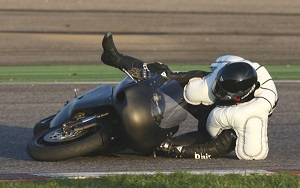
\includegraphics{imagenes/airbag.jpg}
			\caption{Airbag en casco y cazadora}
			\label{contexto:figura}
		\end{figure}
		
		Toda esta información ha sido recopilada de un reportaje de la DGT \cite{Dgt}.
		
		Tal y como hemos podido leer todos estos sistemas en materia de seguridad activa y pasiva son para preveer accidentes o reducir los da\~nos sufridos en caso de accidente. Si el motorista ha sufrido un accidente el tiempo juega en su contra, por lo que se requiere una rápida intervención de los servicios sanitarios. 
		
		Un accidente puede ocurrir en un lugar concurrido y cualquier viandante que se encuentre allí puede realizar dicha llamada a emergencias, el inconveniente sería que el accidente ocurra en una via poco transitada y el conductor no pueda realizar dicha llamada, esperar a que otro conductor circule por esa misma via puede llevar demasiado tiempo.
		
		Como consecuencia nace la realización de este proyecto, cuya aplicación he llamado MotoSafe. Consiste en que el propio smartphone del conductor pueda avisar a emergencias indicándoles nuestra posición en caso que la aplicación haya detectado que se ha producido un accidente a partir de los datos suministrados por el sistema electrónico que ubicaremos en la moto.
		
		En el próximo capítulo se proporcionarán mas detalles acerca del desarrollo de este proyecto.
		
		A continuación detallaré algunos sistemas actuales de alerta móvil en caso de accidentes de tráfico.
		
		\subsection{My-AlarmMe!}
		
			MyAlarmMe! \cite{MyAlamMe} es un sistema de alarma y emergencia para moteros que funciona a través del teléfono móvil.
			
			\begin{figure}[h]
				\centering
				
\includegraphics{imagenes/alarm.JPG}
				\caption{Interfaz de My-AlarmMe}
				\label{contexto:figura}
			\end{figure}
			
			Ofrece un servicio personalizado que permite al usuario avisar, en tiempo real y de forma manual, a todas que personas que el desee con el envío de un SMS que ha sufrido un accidente.
			
			Los sms se enviarán de forma automática al acticar tu alarma, el mensaje enviado será prefijado por el usuario incluyendo el nombre de dicho usuario y las coordenadas de su ubicación.
			
			El funcionamiento es simple, una vez la aplicación ha sido configurada, en caso de sufrir un accidente el usuario solo tiene que abrir la aplicación y pulsar sobre el icono de exclamación, en ese momento se enviarán los sms a los contactos o números previamente indicados.
			
			
		
		\subsection{MEC –- Mobile Emergency Call}
		
			MEC -- Mobile Emergency Call \cite{MEC} es una aplicación que envía mensaje de alarma automaticamente si detecta que hemos tenido un accidente de tráfico. Los mensajes de alerta que envía son por medio de email, SMS y llamada de voz con locución incorporada.
			
			Este sistema se puede usar en coches, motos y bicicletas, teniendo en cuenta las particularidades dinámicas y de conducción de cada vehículo. Si el algoritmo detecta un accidente se inicia una cuenta atrás para enviar los mensajes de alerta, cuenta atrás que puede ser cancelada si el usuario así lo indica.
			
			En esos mensajes de alerta se incluyen la posición GPS del accidente, además de los datos de usuario previamente insertados, como son el modelo de vehículo, alergias conocidas, etcétera. El usuario puede escoger a quien desea enviar dichos mensajes de alerta.
			
			\begin{figure}[h]
				\centering
				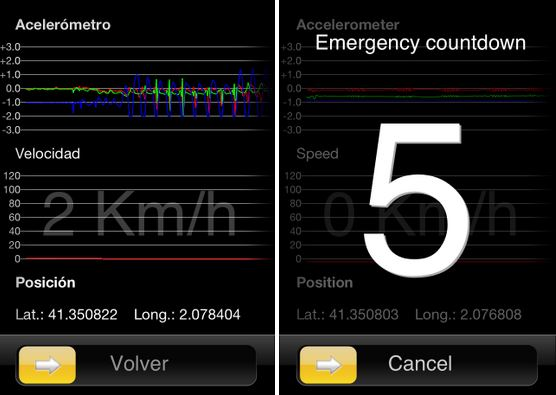
\includegraphics{imagenes/mec.JPG}
				\caption{Interfaz MEC - Mobile Emergency Call}
				\label{contexto:figura}
			\end{figure}
			
		
		
		\subsection{Bosch Media Service}
		
			Bosch \cite{Bosch} ofrece la primera unidad de medición inercial para motocicletas fabricadas en serie. Este sensor proporciona la información necesaria para ofrecer un nivel significativamente mayor de seguridad y comodidad, así como un mayor rendimiento.
			
			Para proporcionar esta información, la unidad de medición inercial MM5.10 mide las señales inerciales 5D, la velocidad de balanceo, la velocidad de viraje, la aceleración longitudinal, la aceleración transversal y la aceleración vertical de la motocicleta. El ángulo de inclinación y el ángulo de cabeceo también se pueden calcular mediante un microcontrolador. La información sobre las velocidades de las ruedas y otros parámetros específicos de la motocicleta (tamaño y forma de los neumáticos y la ubicación de la instalación geométrica del sensor) son necesarios para este cálculo. Todas las señales se transmiten a través de CAN.
			
			Gracias a esta información, es posible obtener y mejorar un gran conjunto de funciones:
				
				\begin{itemize}
					\item Control de tracción
					\item ABS en curvas
					\item Ajuste de wheelie
					\item Ajuste de puesta en marcha
					\item Distribución de la fuerza de frenado en inclinación
					\item Luces de giro
					\item Ajuste del chasis semiactivo
					\item Control en pendientes
					\item Detección de caídas
			    \end{itemize}

	\newpage
	$\ $